% (C) Copyright 2016
% Urs Fässler, www.bitzgi.ch
% SPDX-License-Identifier: CC-BY-SA-4.0

\subsection{Grundlagen}
\label{sec:voraussetzungen}
\subsectionframe

\begin{frame}
	\begin{center}
		\begin{tikzpicture}
		[
			node distance = 3 cm,
			box/.style = {thick, draw=black, top color=white, bottom color=lightblue, rounded corners, align=center, inner sep = 0.5cm},
			can/.style={->, very thick, shorten <=0.2cm, shorten >=0.2cm}
		]
		
		\visible<1-> {
			\node[box] (freedom) {Freie Software};
		}
		
		\visible<2-> {
			\node[box, above right of = freedom] (run) {\only<handout>{1. }Verwenden};
			\draw[can] (freedom) -> (run);
		}
	
		\visible<3-> {
			\node[box, above left of = freedom] (study) {\only<handout>{2. }Verstehen};
			\draw[can]  (freedom) -> (study);
		}
	
		\visible<4-> {
			\node[box, below left of = freedom] (redistribute) {\only<handout>{3. }Verbreiten};
			\draw[can]  (freedom) -> (redistribute);
		}
	
		\visible<5-> {
			\node[box, below right of = freedom] (improve) {\only<handout>{4. }Verbessern};
			\draw[can]  (freedom) -> (improve);
		}
	
		\end{tikzpicture}
	\end{center}
\end{frame}
\note
{
	\footnotesize
	\begin{enumerate}
		\item Die Freiheit, die Software uneingeschränkt und für jeden Zweck einzusetzen.
		\item Die Freiheit, die Funktionsweise der Software untersuchen und verstehen zu können.
		\item Die Freiheit, Kopien der Software zu verbreiten, um damit seinen Mitmenschen zu helfen.
		\item Die Freiheit, die Software zu verbessern und die Verbesserungen an die Öffentlichkeit weiterzugeben, sodass die gesamte Gesellschaft davon profitieren kann.
	\end{enumerate}
	\url{http://www.inf-schule.de/software/freie\_software/02\_freiheiten\_freier\_software}
}

\begin{frame}
	\begin{center}
		\begin{tikzpicture}
		[
			node distance = 2 cm,
			basenode/.style = {thick, draw=black, rounded corners, align=center, inner sep = 0.25cm},
			box/.style = {basenode, top color=white, bottom color=lightblue},
			backbox/.style = {basenode, fill=lightblue!50},
			property/.style={->, very thick, shorten >=0.1cm}
		]
		\small

		\node (center) {};

		\visible<8->{
			\node[box, above = 2.25cm of center] (floss) {FLOSS: Free/Libre Open Source Software};
		}

		\visible<2->{
			\node[box, left = 1.75cm of center] (free) {
\includegraphics[height=1cm]{res/gnu-head.pdf}};
		}
		\visible<3->{
			\node[box, above left of = free] (user) {Anwender};
			\draw[property] (free) -- (user);
			\node[box, above right of = free] (community) {Gesellschaft};
			\draw[property] (free) -- (community);
		}
		\visible<4->{
			\node[box, below left of = free] (ethical) {ethisch};
			\draw[property] (free) -- (ethical);
			\node[box, below right of = free] (social) {sozial};
			\draw[property] (free) -- (social);
		}

		\visible<5->{
			\node[box, right = 1.75cm of center] (open) {
\includegraphics[height=1cm]{res/opensource.pdf}};
		}
		\visible<6->{
			\node[box, above left of = open] (developer) {Entwickler};
			\draw[property] (open) -- (developer);
			\node[box, above right of = open] (business) {Business};
			\draw[property] (open) -- (business);
		}
		\visible<7->{
			\node[box, below left of = open] (practical) {praktisch};
			\draw[property] (open) -- (practical);
			\node[box, below right of = open] (pragmatic) {pragmatisch};
			\draw[property] (open) -- (pragmatic);
		}

		\begin{pgfonlayer}{background} 
			\node[backbox] [fit = (floss) (free) (open) (user) (community) (ethical) (social) (developer) (business) (practical) (pragmatic)] {};
		\end{pgfonlayer}
		
		\end{tikzpicture}
	\end{center}
\end{frame}
\note
{
	\begin{itemize}
		\item \url{https://de.wikipedia.org/wiki/Freie\_Software\#Open\_Source}
		\item A GNU Head: CC-BY-SA Etienne Suvasa \url{https://www.gnu.org/graphics/agnuhead.html}
		\item Logo Open Source Initiative: CC-SA Open Source Initiative official SVG \url{https://commons.wikimedia.org/wiki/File:Opensource.svg}
	\end{itemize}
}

\begin{frame}{Frei und Kommerziell}
	\begin{center}
		\begin{tabular}{c|c|c|}
			 & \visible<3->{\thead{proprietär}} & \visible<2->{\thead{frei}} \\ 
			\hline 
			\visible<4->{\thead{gratis}} & \visible<7->{\makecell{(iOS)\\Freeware}} & \visible<5->{\makecell{Debian\\GNU/Linux}}\\ 
			\hline 
			\visible<4->{\thead{kommerziell}} & \visible<6->{\makecell{Windows\\Mac OS}} & \visible<8->{\makecell{Red Hat Enterprise\\Linux}}\\ 
			\hline 
		\end{tabular} 
	\end{center}
\end{frame}

\begin{frame}{Intellectual Property (IP)}
	\begin{center}
		\visible<2->{\large Geistiges Eigentum}
		\begin{tabular}{ccc}
		\hspace{3cm} & \hspace{3cm} & \hspace{3cm} \\
		\visible<3->{Patent} & \visible<4->{Markenrecht} & \visible<5->{Urheberrecht} \\ 
		\visible<3->{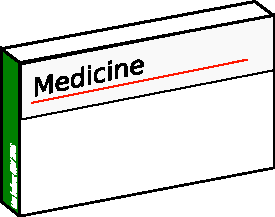
\includegraphics[height=2cm]{res/tulipan-Pharmaceutical-carton.pdf}} & \visible<4->{
\includegraphics[height=2.5cm]{res/gnu-head.pdf}} & \visible<5->{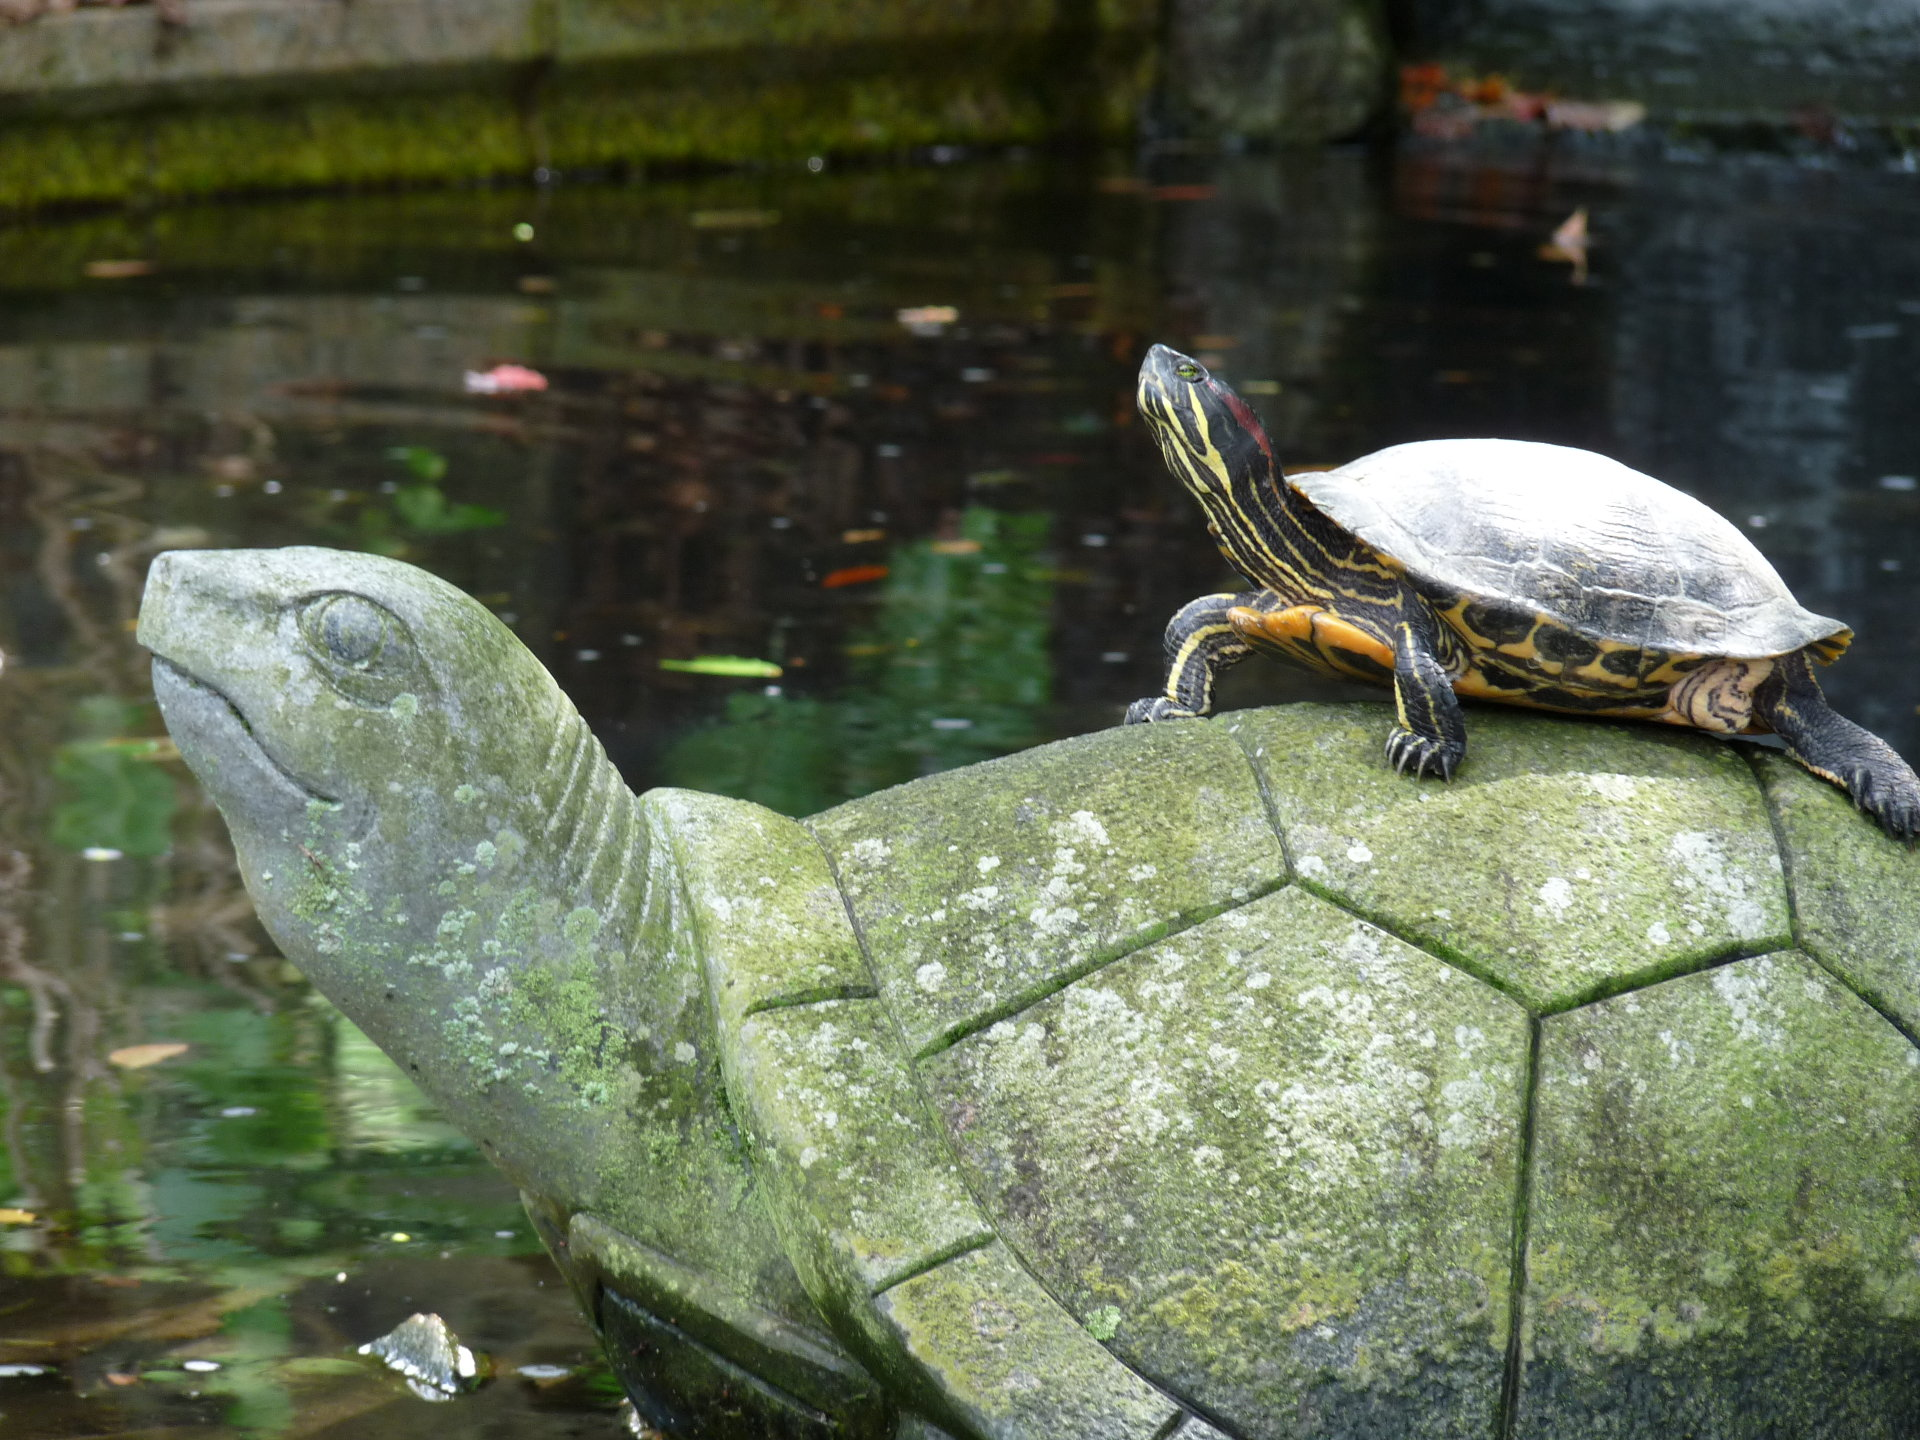
\includegraphics[height=2.5cm]{res/turtles.jpg}} \\ 
		\only<handout>
		{
			\small Auf Antrag & \small Auf Antrag & \small automatisch \\
			\small\makecell{Schutz der\\Investition} & \small\makecell{Schutz von\\Erkennungsmerkmal} & \small\makecell{Verwertungsrecht\\künstlerischer\\Schöpfungen} \\
			\small 20 Jahre & \small beliebig erneuerbar & \small 70 Jahre nach Tod \\
		}
		\end{tabular} 
	\end{center}
\end{frame}
\note
{
	(IP, Intellectual Property, Geistiges Eigentum) \url{https://de.wikipedia.org/wiki/Geistiges\_Eigentum\#Systematik}
	\begin{itemize}
		\item Patent
		\item Markenrecht
		\item Urheberrecht
	\end{itemize}
}
\note
{
	\begin{itemize}
		\item Patent
		\begin{itemize}
			\item \url{https://de.wikipedia.org/wiki/Patent}
			\item Defensivpublikation
			\item Acarton with pills: CC-0 by tulipan \url{https://openclipart.org/detail/6135/pharmaceutical-carton}
		\end{itemize}
	\end{itemize}
}
\note
{
	\begin{itemize}
		\item Markenrecht
		\begin{itemize}
			\item \url{https://de.wikipedia.org/wiki/Marke_(Recht)}
			\item Firefox und Debian (Iceweasel): \url{https://lwn.net/Articles/676799/}
			\item A GNU Head: CC-BY-SA Etienne Suvasa; Trademark of the GNU Project: \url{https://www.gnu.org/graphics/agnuhead.html}
		\end{itemize}
	\end{itemize}
}
\note
{
	\begin{itemize}
		\item Urheberrecht
		\begin{itemize}
			\item \url{https://de.wikipedia.org/wiki/Urheberrecht}
			\item für Werke
			\item daher auch für Software
			\item gilt automatisch: \url{https://anwalt-im-netz.de/urheberrecht/urheberrecht-faq.html\#wann}
			\item Copyrightzeichen ist nicht nötig: \url{https://de.wikipedia.org/wiki/Copyrightzeichen}
			\item Nicht verzichtbar (kein public domain, Gemeinfreiheit: \url{https://de.wikipedia.org/wiki/Gemeinfreiheit\#Entlassung\_in\_die\_Gemeinfreiheit})
		\end{itemize}
	\end{itemize}
}
